\documentclass[11pt,a4paper]{article}

% Packages
\usepackage[utf8]{inputenc}
\usepackage[margin=1in]{geometry}
\usepackage{hyperref}
\usepackage{listings}
\usepackage{xcolor}
\usepackage{fancyhdr}
\usepackage{titlesec}
\usepackage{booktabs}
\usepackage{enumitem}
\usepackage{float}
\usepackage{tikz}
\usetikzlibrary{shapes.geometric, arrows, positioning}

% Colors
\definecolor{codegreen}{rgb}{0,0.6,0}
\definecolor{codegray}{rgb}{0.5,0.5,0.5}
\definecolor{codepurple}{rgb}{0.58,0,0.82}
\definecolor{backcolour}{rgb}{0.95,0.95,0.92}

% Code listing style
\lstdefinestyle{mystyle}{
    backgroundcolor=\color{backcolour},
    commentstyle=\color{codegreen},
    keywordstyle=\color{magenta},
    numberstyle=\tiny\color{codegray},
    stringstyle=\color{codepurple},
    basicstyle=\ttfamily\footnotesize,
    breakatwhitespace=false,
    breaklines=true,
    captionpos=b,
    keepspaces=true,
    numbers=left,
    numbersep=5pt,
    showspaces=false,
    showstringspaces=false,
    showtabs=false,
    tabsize=2
}
\lstset{style=mystyle}

% Header and footer
\pagestyle{fancy}
\fancyhf{}
\rhead{Transport Reliability Analytics}
\lhead{Technical Report}
\rfoot{Page \thepage}

% Hyperlink setup
\hypersetup{
    colorlinks=true,
    linkcolor=blue,
    filecolor=magenta,
    urlcolor=cyan,
}

% TikZ styles
\tikzstyle{component} = [rectangle, rounded corners, minimum width=2.5cm, minimum height=1cm, text centered, draw=black, fill=blue!20]
\tikzstyle{database} = [cylinder, shape border rotate=90, aspect=0.25, minimum width=2.5cm, minimum height=1cm, text centered, draw=black, fill=green!20]
\tikzstyle{arrow} = [thick,->,>=stealth]

\begin{document}

% Title Page
\begin{titlepage}
    \centering
    \vspace*{2cm}
    {\Huge \textbf{Transport Reliability Analytics}}\\[0.5cm]
    {\Large Technical Report}\\[2cm]

    {\large \textbf{Land Transport Authority (LTA)}}\\[0.3cm]
    {\large Singapore MRT \& Bus Network}\\[2cm]

    \begin{tabular}{ll}
        \textbf{Stack:} & Go, gRPC, PostgreSQL, Next.js \\
        \textbf{Deployment:} & Docker Compose \\
    \end{tabular}\\[3cm]

    {\large \today}
    \vfill
\end{titlepage}

% Table of Contents
\tableofcontents
\newpage

% Executive Summary
\section{Executive Summary}

This document provides an overview of the Transport Reliability Analytics system - a production-ready full-stack application for tracking and analyzing transport incidents across Singapore's MRT and bus network.

\subsection{Quick Start}

Start the entire system with one command:
\begin{lstlisting}[language=bash]
docker-compose up
\end{lstlisting}

Access the dashboard at: \url{http://localhost:3000}

\section{System Architecture}

\subsection{Component Diagram}

\begin{figure}[H]
\centering
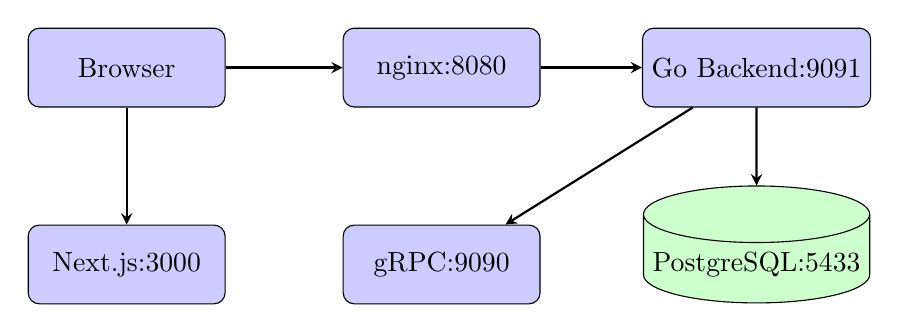
\begin{tikzpicture}[node distance=2cm]
% Nodes
\node (browser) [component] {Browser};
\node (nginx) [component, right of=browser, xshift=2cm] {nginx\\:8080};
\node (backend) [component, right of=nginx, xshift=2cm] {Go Backend\\:9091};
\node (db) [database, below of=backend, yshift=-0.5cm] {PostgreSQL\\:5433};
\node (frontend) [component, below of=browser, yshift=-0.5cm] {Next.js\\:3000};
\node (grpc) [component, below of=nginx, yshift=-0.5cm] {gRPC\\:9090};

% Arrows
\draw [arrow] (browser) -- (nginx);
\draw [arrow] (nginx) -- (backend);
\draw [arrow] (backend) -- (db);
\draw [arrow] (browser) -- (frontend);
\draw [arrow] (backend) -- (grpc);
\end{tikzpicture}
\caption{System Architecture}
\end{figure}

\subsection{Technology Stack}

\textbf{Backend:} Go 1.24, go-coldbrew, gRPC, PostgreSQL 15

\textbf{Frontend:} Next.js 15, React 18, TypeScript, Tailwind CSS

\textbf{Infrastructure:} Docker, nginx

\section{Getting Started}

\subsection{Prerequisites}
\begin{itemize}[leftmargin=*]
    \item Docker and Docker Compose
    \item Ports 3000, 8080, 9090, 9091, 5433 available
\end{itemize}

\subsection{Installation}

\textbf{Automated Setup:}
\begin{lstlisting}[language=bash]
./setup.sh
\end{lstlisting}

\textbf{Manual Setup:}
\begin{lstlisting}[language=bash]
docker-compose up
\end{lstlisting}

\subsection{Access Points}

\begin{table}[H]
\centering
\begin{tabular}{@{}lll@{}}
\toprule
\textbf{Service} & \textbf{URL} & \textbf{Port} \\ \midrule
Dashboard & \url{http://localhost:3000} & 3000 \\
API & \url{http://localhost:8080} & 8080 \\
Backend & \url{http://localhost:9091} & 9091 \\
Database & localhost:5433 & 5433 \\ \bottomrule
\end{tabular}
\end{table}

\section{API Documentation}

\subsection{Endpoints}

\begin{table}[H]
\centering
\small
\begin{tabular}{@{}llp{6cm}@{}}
\toprule
\textbf{Method} & \textbf{Endpoint} & \textbf{Description} \\ \midrule
POST & /incidents & Submit new incident \\
GET & /analytics/top\_breakdowns & Top N lines/stations \\
GET & /analytics/mean\_time\_between\_failures & MTBF calculation \\
GET & /analytics/recent\_disruptions & Recent incidents \\ \bottomrule
\end{tabular}
\end{table}

\subsection{Example: Create Incident}

\begin{lstlisting}[language=bash]
curl -X POST http://localhost:8080/incidents \
  -H "Content-Type: application/json" \
  -d '{
    "line": "North South Line",
    "station": "Orchard",
    "timestamp": "2025-10-16T08:32:00Z",
    "duration_minutes": 45,
    "incident_type": "signal"
  }'
\end{lstlisting}

\subsection{Example: Get Top Breakdowns}

\begin{lstlisting}[language=bash]
curl "http://localhost:8080/analytics/top_breakdowns?scope=station&limit=5"
\end{lstlisting}

\section{Database Schema}

\subsection{Tables}

\textbf{lines:} id (UUID), name (TEXT), created\_at

\textbf{stations:} id (UUID), name (TEXT), line\_id (FK), status, created\_at

\textbf{incidents:} id (UUID), station\_id (FK), line\_id (FK), ts, duration\_minutes, incident\_type, status

\subsection{Performance Indexes}

\begin{itemize}[leftmargin=*]
    \item \texttt{idx\_incidents\_ts} - Timestamp descending
    \item \texttt{idx\_incidents\_line\_ts} - Line + timestamp (covering index)
    \item \texttt{idx\_incidents\_station\_ts} - Station + timestamp (covering index)
    \item \texttt{idx\_incidents\_status} - Status filtering
\end{itemize}

\subsection{Seed Data}

\begin{itemize}[leftmargin=*]
    \item 6 MRT lines (NSL, EWL, CCL, DTL, TEL, NEL)
    \item 150+ stations
    \item 400+ incidents (last 90 days)
\end{itemize}

\section{Performance Testing}

\subsection{Stress Test Results}

Two load tests were performed to validate system performance under real conditions:

\textbf{Light Load Test (10 QPS):}
\begin{table}[H]
\centering
\begin{tabular}{@{}lr@{}}
\toprule
\textbf{Metric} & \textbf{Result} \\ \midrule
Total Requests & 600 \\
Success Rate & 100\% \\
Mean Latency & 5.2ms \\
p50 Latency & 5.1ms \\
p95 Latency & 9.4ms \\
p99 Latency & 11.2ms \\ \bottomrule
\end{tabular}
\end{table}

\textbf{Heavy Load Test (100 QPS):}
\begin{table}[H]
\centering
\begin{tabular}{@{}lr@{}}
\toprule
\textbf{Metric} & \textbf{Result} \\ \midrule
Total Requests & 6,000 \\
Success Rate & 100\% \\
Mean Latency & 3.0ms \\
p50 Latency & 2.6ms \\
p95 Latency & 6.0ms \\
p99 Latency & 8.0ms \\ \bottomrule
\end{tabular}
\end{table}

\subsection{Running Tests}

\begin{lstlisting}[language=bash]
# Run all stress tests
make stress-test

# Individual tests
make stress-test-10qps
make stress-test-100qps
\end{lstlisting}

\section{Frontend Dashboard}

\subsection{Features}
\begin{itemize}[leftmargin=*]
    \item Auto-refresh every 30 seconds
    \item Interactive bar charts (top breakdowns)
    \item Color-coded MTBF metrics
    \item Sortable disruptions table
    \item Manual refresh button
\end{itemize}

\subsection{Technology}
Next.js 15, TypeScript, Tailwind CSS, Recharts

\section{Production Considerations}

\subsection{Scaling}
\begin{itemize}[leftmargin=*]
    \item Horizontal: Multiple app instances behind load balancer
    \item Database: Read replicas for analytics
    \item Connection pooling: 25 max, 5 idle
\end{itemize}

\subsection{Monitoring}
\begin{itemize}[leftmargin=*]
    \item Health checks: \texttt{/health} and \texttt{/ready}
    \item Structured logging with request IDs
    \item Prometheus metrics endpoint
\end{itemize}

\subsection{Security}
\begin{itemize}[leftmargin=*]
    \item Change default passwords
    \item Enable SSL/TLS
    \item Implement API authentication
    \item Add rate limiting
    \item CORS via nginx
\end{itemize}

\section{Troubleshooting}

\subsection{Common Issues}

\textbf{Port Conflicts:} Edit \texttt{docker-compose.yml} to change ports

\textbf{Database Issues:}
\begin{lstlisting}[language=bash]
docker-compose logs db
docker-compose exec db psql -U lta_user -d transport_reliability
\end{lstlisting}

\textbf{Frontend API Errors:}
\begin{enumerate}[leftmargin=*]
    \item Verify nginx: \texttt{docker-compose ps nginx}
    \item Test API: \texttt{curl http://localhost:8080/health}
    \item Hard refresh browser: Cmd+Shift+R
\end{enumerate}

\section{Conclusion}

The Transport Reliability Analytics system is a production-ready application demonstrating:

\begin{itemize}[leftmargin=*]
    \item Modern microservices architecture
    \item High-performance API (100+ QPS)
    \item Real-time data visualization
    \item Professional Docker deployment
\end{itemize}

\subsection{Project Structure}

\begin{lstlisting}
.
├── backend/          # Go services
├── database/         # PostgreSQL setup
├── frontend/         # Next.js dashboard
├── nginx/            # Reverse proxy
├── proto/            # Protocol buffers
├── scripts/          # Stress tests
└── docker-compose.yml
\end{lstlisting}

\vspace{1cm}

\noindent
\textbf{Repository:} \texttt{stunning-octo-eureka}

\noindent
\textbf{Tech Stack:} Go · gRPC · PostgreSQL · Next.js · Docker · nginx

\end{document}
